
\section{Bayesian concepts}

\begin{frame}{The likelihood approach}

	\begin{block}{}
		\begin{itemize}
			\item $Y$ is a random variable
			\item $f({y}|{\theta})$ is a probability distribution (called 
			the \textit{likelihood}) representing the sampling model for the observed 
			data $(y_1,y_2,...,y_n)$ given a vector of unknown parameters ${\theta}$
			\item $\int f({y}|{\theta})d{\theta}$ is not necessarily $=1$ or even finite
			\item It is possible to find the value of ${\theta}$ that maximises the 
			likelihood function: we can calculate 
			a \textit{maximum likelihood estimate} (MLE) for ${\theta}$, as: 
			$\hat{{\theta}}=argmax_{{\theta}}f({y}|{\theta})$
		\end{itemize}
	\end{block}

\end{frame}


\begin{frame}{Bayes' Theorem}

	\begin{block}{}
		\begin{equation}
			p({\theta}|{y}) = \frac{f({y}|{\theta})\pi({\theta})}{m({y})} = \frac{f({y}|{\theta})\pi({\theta})}{\int f({y}|{\theta})\pi({\theta}) d{\theta}}
		\end{equation}
	\end{block}

	\begin{itemize}
		\item ${\theta}$ is not a fixed parameter but a random quantity with 
		prior distribution $\pi({\theta})$
		\item $p({\theta}|{y})$ is the posterior probability distribution of ${\theta}$
		\item $\int p({\theta}|{y})d{\theta}=1$
	\end{itemize}

\end{frame}

\begin{frame}{Bayes' Theorem in action!}

	\begin{figure}[!ht]
		\centering
		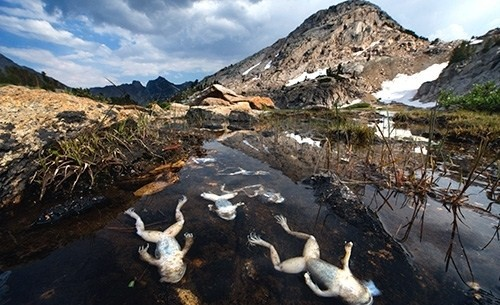
\includegraphics[width=6cm]{Images/Frogs.jpg}
		\caption{The chytrid fungus \textit{Batrachochytrium dendrobatidis} is the most 
		significant threat to amphibians.}
		\label{Fig:Frogs}
	\end{figure}

	Let's prove Bayes' Theorem!

\end{frame}

\begin{frame}{Venn diagrams}

	\begin{figure}[!ht]
		\centering
		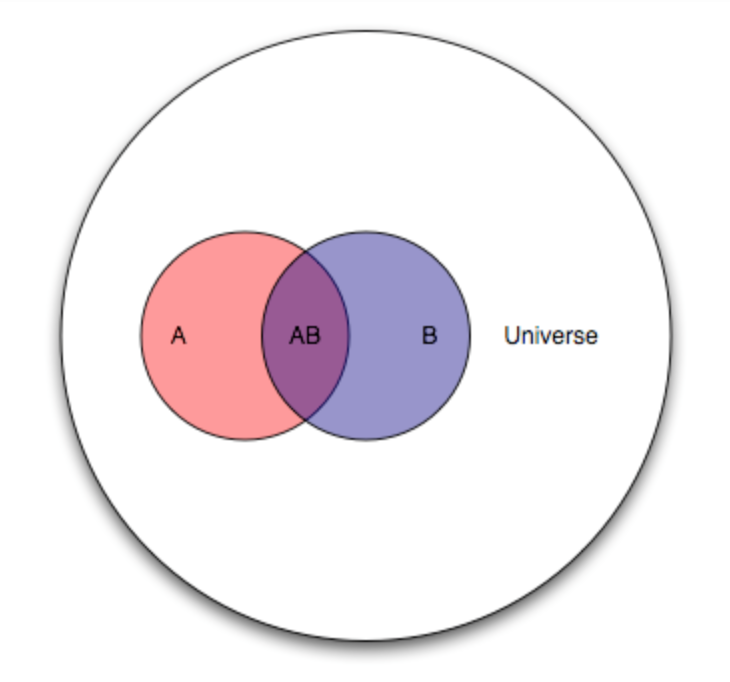
\includegraphics[width=4cm]{Images/Set3.png}
		\caption{Sets $U$, $A$ (samples with infection), $B$ (samples with positive test 
		result) and $A \cap B$ (or $AB$).}
		\label{Fig:Set3}
	\end{figure}

	Given that the test is positive for a randomly selected sample, what is the probability 
	that said sample is infected?

\end{frame}

\begin{frame}{Normal-Normal model}

	\begin{block}{}
		If
		\begin{align}
			f(y|\theta) &= N(y|\theta, \sigma^2)\\
			\pi(\theta) &= N(\theta|\mu, \tau^2)
		\end{align}
		then
		\begin{equation}
			p(\theta|y) = N(\theta|\frac{\sigma^2\mu+\tau^2y}{\sigma^2+\tau^2},\frac{\sigma^2\tau^2}{\sigma^2 + \tau^2})
		\end{equation}
	\end{block} 

\end{frame}

\begin{frame}{Normal-Normal model}

	\begin{block}{"Shrinking" factor $B$}
		\begin{equation}
			B = \frac{\sigma^2}{\sigma^2+\tau^2}
		\end{equation}
		with $0 \leq B \geq 1$. \\Then
		\begin{align}
			E(\theta|y) &= B\mu + (1-B)y\\
			Var(\theta|y) &= (1-B)\sigma^2 \equiv B\tau^2
		\end{align}
	\end{block} 

	\pause

	Question:\\
	\begin{itemize}
		\item What if $\sigma^2>>\tau^2$?
		\item What if $\sigma^2<<\tau^2$?
	\end{itemize}

\end{frame}

\begin{frame}{Save the frogs with a Normal-Normal model!}

	\begin{block}{Infected frogs (observed and "believed" \textit{a priori})}
		Assume that $y=6$, $\sigma=1$, $\mu=2$ and $\tau=1$.
	\end{block}

	 \begin{align}
         	f(y=6|\theta) &= N(y=6|\theta, 1)\\
              	\pi(\theta) &= N(\theta|2, 1)
	\end{align}

	\pause
	
	Exercise:\\
	\begin{enumerate}
		\item Open \texttt{R} and calculate and plot the prior, likelihood, 
		and posterior distribution.
		\item Calculate the \textit{maximum a posteriori probability} (MAP).
		\item What happens if we use a skewer (sharper) or wider prior?
		\item What happens if we have more observations?
	\end{enumerate}

\end{frame}

\begin{frame}{Monte Carlo sampling}

	Drawing random samples from the posterior distribution instead of calculating its parameters.

	\begin{figure}[!ht]
		\centering
		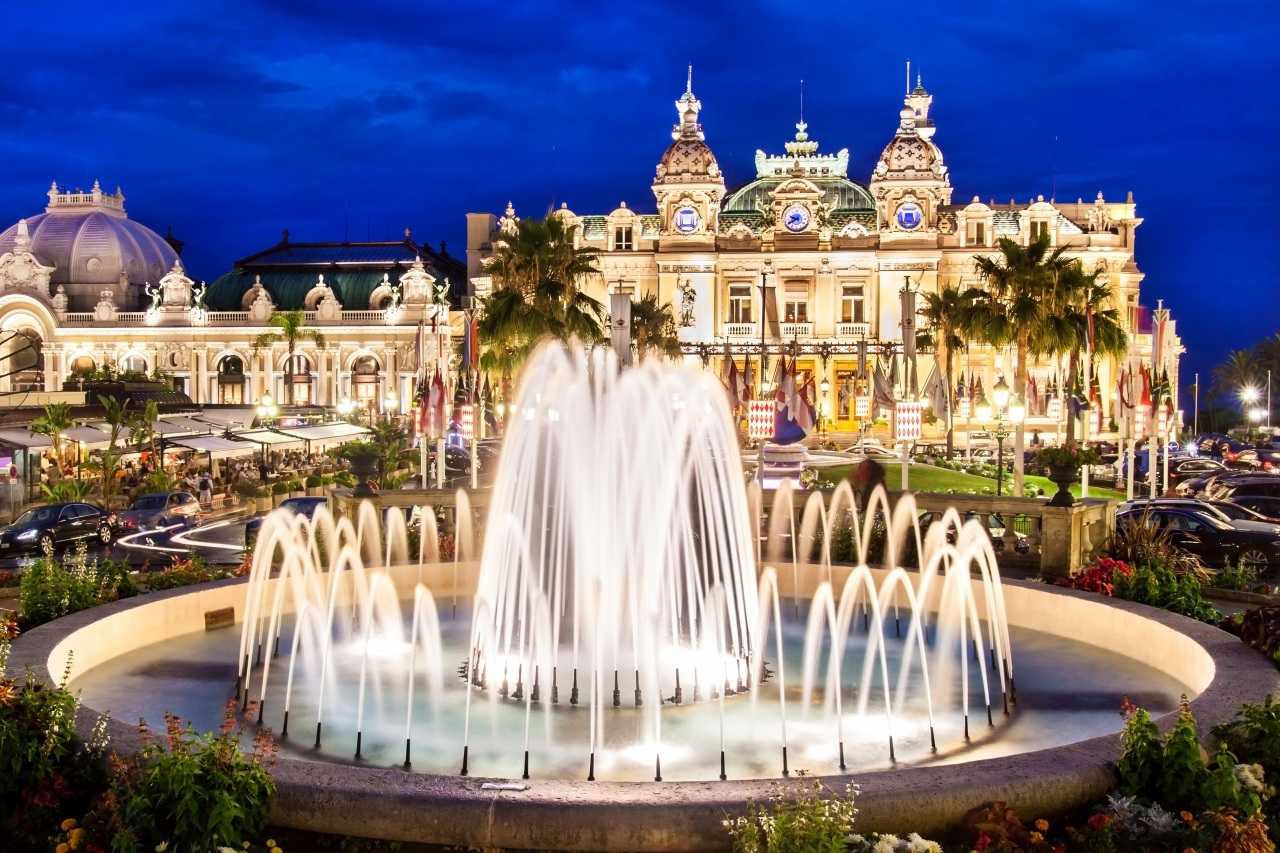
\includegraphics[width=4cm]{Images/MonteCarlo.jpeg}
		\caption{Monte Carlo and its famous casino.}
		\label{Fig:MonteCarlo}
	\end{figure}

	Exercise:\\
	\begin{enumerate}
		\item Open \texttt{R} and plot the posterior distribution of the previous example 
		using Monte Carlo sampling.
		\item What happens if we use more or less samples?
	\end{enumerate}

\end{frame}



